\chapter{Inleiding}

Het internet zoals we het vandaag kennen is niet meer weg te denken en het aantal aangesloten machines blijft groeien. Tot voor kort bestond deze verzameling machines uit computers, routers, etc... en bijna alle data die het huidige internet omvat werd ingevoerd door menselijke tussenkomst.
Maar daar komt verandering in. De aangesloten machines evolueren naar objecten of 'dingen', waarbij elk object uniek adresseerbaar is en zelf data kan inbrengen zonder menselijke tussenkomst. Deze objecten kunnen allerlei apparaten voorstellen, van een smartphone tot een wasmachine of zelfs een auto.\\

\begin{wrapfigure}{r}{0.5\textwidth}
\vspace{-10pt}
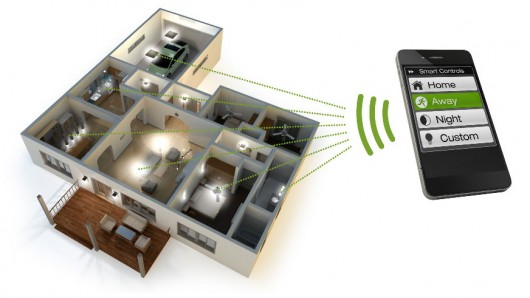
\includegraphics[width=0.48\textwidth]{fig/InternetOfThings}
\vspace{-10pt}
\caption{Internet of Things}
\vspace{-10pt}
\end{wrapfigure}
De komende jaren zal de omvang van het Internet exploderen omdat steeds meer van deze dagdagelijkse objecten ermee verbonden worden. Het Internet zal evolueren naar een \textit{Internet of Things} (IoT)\nomenclature{IoT}{Internet of Things} en zal ons toelaten om op een eenvoudige manier en van op afstand informatie te verkrijgen over apparaten en hun omgeving (bv. de temperatuur, een deurslot, de status van de wasmachine) en ermee te interageren (bv. sluiten van de deur, aanschakelen van de verwarming). Tot voor kort was het besturen van apparaten in je huis vanop afstand met een smartphone, computer, etc slechts een theorie, maar de realisatie hiervan is nu dichter dan ooit.

\subsubsection{Is het internet klaar voor het IoT?}
Een grote remming op de ontwikkeling van een IoT is het beperkte adresbereik van Internet Protocol versie 4 (IPv4)\nomenclature{IPv4}{Internet Protocol versie 4}, maar met de invoering van Internet Protocol versie 6 (IPv6)\nomenclature{IPv6}{Internet Protocol versie 6} voor de deur, wordt het aantal mogelijke adressen aanzienlijk groter.
Alhoewel IPv6 voldoet aan de eisen voor het IoT zal de invoering van IPv6 op grote schaal nog even op zich laten wachten. Daarom zal het IoT voorlopig beperkt blijven tot testomgevingen en netwerken op kleinere schaal.\\
Een tweede probleem wordt gevormd door het verkeer dat zo'n sensornetwerk veroorzaakt. Huidig gebruikte protocollen zoals HTTP zijn niet geoptimaliseerd voor verkeer in en uit een sensornetwerk. Er zijn wel nieuwe protocollen ontwikkelt voor deze taak maar die zijn nog niet ingeburgerd.\\
De conclusie is dat het Internet in het geheel en onder zijn huidige vorm nog niet klaar is voor het IoT, maar dat niets in de weg staat van de ontwikkeling ervan in de zeer nabije toekomst.

\section{Doel}
Omwille van deze evolutie worden er meer en meer embedded devices ontwikkeld voor het IoT. Onder embedded devices verstaan we devices waar resources op aangesloten zijn. Het device biedt deze resources aan, aan de buitenwereld. Deze masterproef behandelt voornamelijk de integratie van die embedded devices in bestaande systemen. De focus ligt dan niet zozeer op de ontwikkeling van de embedded devices zelf, maar op het aanspreken en besturen ervan. Meer specifiek willen we een bijdrage leveren aan de realisatie van webservices voor het IoT. Het vertrekpunt hiervoor zullen de recente CoAP-ontwikkelingen zijn van de iMinds-onderzoeksgroep (C++ CoAP framework, HTTP/CoAP-proxy, CoAP voor sensoren…). Als embedded device gebruiken we sensoren aangeboden door iMinds die bereikbaar zijn onder de vorm van een sensornetwerk.\\

Deze webservice bieden we aan onder de vorm van een Drupalmodule waarbij een gebruiker een device rechtstreeks op locatie kan aanspreken door middel van native CoAP-communicatie zonder dat er een proxy aan te pas komt. Dit is een groot verschil met recente implementaties waarbij er gebruik gemaakt wordt van een HTTP/CoAP-proxy tussen de applicatie en het device. Concreet worden er twee modules ontwikkeld. Een CoAP-\textit{library} die al het CoAP-verkeer stuurt en afhandelt en een CoAP-sensormodule waarin de gegevens afkomstig van de devices, verwerkt en weergegeven worden. De modules moeten zo ontwikkeld worden dat ze op een eenvoudige manier te gebruiken zijn, zodat geen kennis van de technische aspecten vereist is.

\section{Verloop masterproef}
%Voor de eigenlijke ontwikkeling van de Drupalmodule werden verscheidene boeken geraadpleegd \cite{beginDrupal, proDrupal, drupalDefGuide}, waarbij voor de implementatiedetails van CoAP, de CoAP-drafts werden geraadpleegd \cite{coapDraft, coapObserveDraft, coapConditionalObserveDraft, coapDiscovery, blockwiseTransfer, coreInterfaces}.\\
%In een eerste fase van deze masterproef zal de Drupalmodule wel nog gebruik maken van een HTTP/CoAP-proxy. Wanneer deze eerste fase geoptimaliseerd is, wordt de proxy uitgesloten en wordt er enkel nog gebruik gemaakt van CoAP.\\

Na een uitgebreide literatuurstudie van Drupal en PHP Hypertext Preprocessor (PHP, de gebruikte programmeertaal)\nomenclature{PHP}{PHP Hypertext Preprocessor} werd gepoogd een testmodule te maken. Het resultaat van deze eerste module bestond uit een webservice die dynamisch kon worden toegevoegd aan een Drupal website. Men kon deze webservice aanwenden om aan de hand van een Where On Earth ID (WOEID)\nomenclature{WOEID}{Where On Earth ID}, het weerbericht op te vragen van een plaats naar keuze.\\
De volgende stap bestond uit de ontwikkeling van een eerste versie van de uiteindelijk te ontwikkelen module. Deze bood de gebruiker de mogelijkheid om de waarde van \'{e}\'{e}n resource op te vragen. Bovendien kon de gebruiker met een checkbox aangeven of de waarde periodiek moest worden opgehaald. De opgehaalde waarden werden getoond in een tabel. In deze fase werd er nog gebruik gemaakt van een HTTP/CoAP-proxy. Later wordt de proxy uitgesloten en wordt er enkel nog gebruik gemaakt van CoAP.\\
Na uitvoerig bestuderen van de CoAP-drafts en het ontmantelen van CoAP-berichten in Wireshark \cite{wireshark}, werd ge\"{e}xperimenteerd met CoAP-berichten (Wireshark is een network sniffer). Al vlug bleek dat de ontwikkeling van een eigen CoAP-\textit{library} geschreven in PHP, de beste oplossing was. Aldus werd een aparte module ontwikkeld, een CoAP-\textit{library} die alle CoAP-communicatie voor zich neemt. Deze module biedt de mogelijkheid tot opstellen, versturen en ontvangen van CoAP-berichten.\\
Met de CoAP-\textit{library} voorhanden werd het nu mogelijk de CoAP-sensormodule aan te passen zodat die enkel nog gebruik maakt van CoAP-communicatie. Door deze laatste ontwikkeling werd ook de observe-methode van CoAP mogelijk, welke later toegelicht wordt in paragraaf \ref{observe}.\\
Naast deze laatste ontwikkelingen die zich eerder toespitsen op de \textit{backend}, werd ook vooruitgang geboekt op de \textit{frontend}. Er werd ingespeeld op de mogelijkheden van Drupal zodat een gebruiker gemakkelijk een CoAP-resource kan toevoegen aan zijn/haar website.\\
Omdat een gebruiker soms niet weet welke resources allemaal aangesloten zijn op een embedded device, wordt resource discovery voorzien. Dit houdt in dat de gebruiker enkel het IPv6 adres moet opgeven van een embedded device, waarna een lijst zal worden gegenereerd en getoond die alle resources bevat, aangesloten op dat embedded device.\\
Dit laatste concept kan nog verder worden doorgedreven tot het concept van service discovery. Hierbij krijgt de gebruiker een overzicht van lijsten van resources van elk embedded device in een bepaald subnetwerk. Als alternatief zien wij een resource directory \cite{coapDraft, coapDiscovery}. Deze wordt ge\"{i}mplementeerd op een specifieke machine waar alle embedded devices hun core op beschikbaar stellen. Een gebruiker kan deze directory aanroepen om toegang te krijgen tot alle well-known/cores. De integratie met een resource directory werd echter niet ge\"{i}mplementeerd, maar wordt in deze scriptie wel behandeld als mogelijke uitbreiding (Zie paragraaf \ref{resourceDirectory}).\\
Als laatste stap rest ons nog het samenvoegen van de \textit{frontend} en \textit{backend}. Als resultaat bekomt men dan een gebruiksvriendelijke module die de gebruiker in staat stelt sensoren te bekijken en te beheren zonder daarvoor enige kennis van onderliggende technologie\"{e}n nodig te hebben.


\section{Structuur scriptie}
Hoofdstuk twee handelt over Drupal. We geven de voor- en nadelen van Drupal en gaan dieper in op enkele van de belangrijkste concepten en termen. We bekijken eveneens beknopt de werking van Drupal. Als laatste onderdeel van dit hoofdstuk bespreken we een voorbeeld van een Drupal module waarin jQuery gebruikt wordt.\\

In hoofdstuk drie gaan we dieper in op de concepten en mogelijkheden van CoAP. We bekijken het berichtformaat van CoAP en geven een vergelijking met HTTP. De voor- en nadelen komen eveneens aan bod. We bespreken de verschillende soorten communicatie en gaan ook dieper in op de concepten die met resource discovery te maken hebben. Deze concepten staan centraal in het automatiseren van ophalen van sensorgegevens.\\

In het vierde hoofdstuk bespreken we de ontwikkelde CoAP-\textit{library}. Het ontwikkelingsproces wordt hier uitvoerig besproken, waarbij struikelpunten worden aangegeven en de gemaakte keuzes worden verantwoord. We bekijken ook de aangeboden functionaliteiten.\\

In het vijfde hoofdstuk bespreken we de CoAP-sensormodule. Er wordt grondig ingegaan op de architectuur van de module. Tevens wordt de evolutie van de module behandeld, er zijn namelijk verschillende versies ontwikkeld in de loop van de masterproef. Het eindresultaat wordt uitvoerig besproken.\\

Het zesde en laatste hoofdstuk handelt over mogelijke uitbreidingen die wij nog graag hadden ge\"{i}mplementeerd maar niet meer pasten in de tijd die voorzien was. We sommen deze op en lichtten toe welke implementatie wij voor ogen hadden.










